%%
% This is an Overleaf template for Master's and Bachelor's theses
% using the TUM Corporate Design https://www.tum.de/cd
%
% For further details on how to use the template, take a look at our
% GitLab repository and browse through our test documents
% https://gitlab.lrz.de/latex4ei/tum-templates.
%
% The tumbook class is based on the KOMA-Script class scrbook.
% If you need further customization please consult the KOMA-Script guide
% https://ctan.org/pkg/koma-script.
% Additional class options are passed down to the base class.
%
% If you encounter any bugs or undesired behaviour, please raise an issue
% in our GitLab repository
% https://gitlab.lrz.de/latex4ei/tum-templates/issues
% and provide a description and minimal working example of your problem.
%%


\documentclass[
  a4paper,            % paper size (a4paper, a5paper)
  thesis=student,     % define the type of the thesis (student, phd, none)
  english,            % define the document language (english, german)
  % BCOR=5mm,           % define a binding offset for the document
  % coverBCOR=1cm,      % define a different binding offset for the cover page
  coverpage=false,    % disable the cover page (e.g. if a tumcover is used)
  titlepage=false,    % disable the additional title page
  oneside,            % use onesided or twosided layout (oneside, twoside)
  % headmarks=true,     % enable headmarks (true, false)
  font=times          % define main text font (helvet, times, palatino, libertine)
]{tumbook}

% For theses that are printed with a transparent cover it is recommended to
% use the coverpage and provide the proper coverBCOR, so the distance between
% the binding strip and the content is properly set to 1 * logoheight.
% In this case, the publisher and titleback information is most certainly
% empty and the titlepage may be turned off.
%
% For theses that are printed with a soft cover or by a publisher it is
% recommended to create a cover using the tumcover class and therefore turn
% off the coverpage here. In this case, you most certainly have publisher and
% titleback information and you should keep the titlepage option enabled.


% load additional packages
\usepackage{listings}
\usepackage{tikz}
\usepackage{graphicx}
\usepackage{multirow}
\usepackage{rotating}
\usepackage{array}
\usepackage{caption}
\usepackage{booktabs}
\usepackage{tabularx}
\usepackage{longtable}

\lstset{
    language=C,
    basicstyle=\ttfamily\small,
    numbers=left,
    numberstyle=\tiny,
    stepnumber=1,
    numbersep=5pt,
    backgroundcolor=\color{lightgray},
    showspaces=false,
    showstringspaces=false,
    showtabs=false,
    frame=single,
    tabsize=2,
    captionpos=b,
    breaklines=true,
    breakatwhitespace=false,
}


% thesis metadata
\title{Evaluation of OpenASIP Custom Operations in CoreDSL Ecosystem}
\subtitle{}
\author{Hengsheng Li}

\degree{Bachelor of Science (B.Sc.)}
\dateSubmitted{18.10.2024}

\examiner{Prof.\@~Dr.-Ing.\@ Ulf Schlichtmann}
\supervisor{M.Sc. Philipp van Kempen}


\begin{document}

\frontmatter
\maketitle
\chapter{Abstract}
This thesis evaluates the integration and performance improvement of custom operations designed using the OpenASIP 2.0 Co-Design toolchain within the CoreDSL ecosystem, leveraging the Extendable Translating Instruction Set Simulator (ETISS). As hardware-software co-design becomes increasingly crucial in the optimization of modern embedded systems, custom instructions tailored to specific applications can significantly enhance performance. This research systematically collected and translated OpenASIP-defined custom operations into CoreDSL syntax to create a pipeline for generating ETISS-compatible architectures. These architectures were evaluated against a series of benchmarks using the MLonMCU framework, a tool designed for benchmarking machine learning workloads on microcontrollers. In this study, we delve into the intricacies of translating complex custom operations and the corresponding challenges within the CoreDSL environment, examining the effectiveness of ETISS in simulating these architectures. Through comprehensive benchmarking, we demonstrate that custom instructions, when effectively integrated, can yield up to 28\% performance improvements over the baseline, reflecting the potential of custom operations in enhancing application-specific workloads.
\tableofcontents

\mainmatter
\chapter{Introduction}
RISC-V, an open-source instruction set architecture (ISA), has seen widespread adoption across various domains due to its modular design and open nature.
Its applications span embedded systems, where it powers devices like sensors and microcontrollers, and consumer electronics, including smartphones and smartwatches.
In automotive technology, RISC-V is being integrated into advanced driver-assistance systems (ADAS) and infotainment units. Additionally,
its flexibility makes it a popular choice in academic research for processor design and computer architecture experimentation.
The versatility and open-source model of RISC-V facilitate innovation and customization, driving advancements in numerous technological sectors.

To leverage this flexibility effectively, simulation and validation of custom instructions are essential.
The ETISS (Extendable Translating Instruction Set Simulator) \cite{ETISS} provides a robust platform for instruction set simulation,
offering the capability to model and test custom processor architectures.
However, to fully utilize ETISS's capabilities, it is beneficial to integrate it with a flexible tool for defining custom instructions.

OpenASIP 2.0 \cite{OpenASIP} is a co-design toolset designed to facilitate the customization of RISC-V-based processors,
supporting RTL generation and high-level programming of custom instructions.
By translating OpenASIP's custom instruction sets into CoreDSL \cite{CoreDSL} syntax—a descriptive language for hardware design—we can enhance the integration with ETISS.
CoreDSL allows for a clear and flexible specification of custom instructions,
which can be seamlessly applied to ETISS for comprehensive simulation and evaluation.

Thus, this paper focuses on translating OpenASIP's custom instruction sets into CoreDSL language and applying them within the ETISS framework.
This approach aims to streamline the process of integrating and evaluating custom instructions,
ultimately improving the effectiveness and efficiency of the simulation environment for RISC-V processors.

\chapter{State of the Art}
\section{Existing Solutions and Approaches}

\begin{enumerate}

    \item \textbf{RISC-V ISA Extensions:}
    The RISC-V instruction set architecture (ISA) has gained significant traction due to its open-source and modular design, allowing extensive customization.
    Recent research has provided a survey of RISC-V ISA extensions, covering various improvements and customizations aimed at enhancing processor performance and capabilities \cite{Risc-v}.

    \item \textbf{ETISS (Extendable Translating Instruction Set Simulator):}
    ETISS \cite{ETISS} is a prominent tool for instruction set simulation, enabling detailed modeling and evaluation of custom processor architectures.
    It supports functional and performance simulations but is designed to work with CoreDSL-based instruction sets. Integrating custom instructions from other formats poses challenges.

    \item \textbf{OpenASIP 2.0:}
    OpenASIP 2.0 \cite{OpenASIP} is a co-design toolset for customizing RISC-V processors, providing features for RTL generation and programming of custom instructions.
    While effective for defining and validating custom instructions, it lacks direct support for integration with ETISS, which uses CoreDSL for instruction definitions.

    \item \textbf{CoreDSL:}
    CoreDSL \cite{CoreDSL} is a descriptive language for hardware design, including custom instructions.
    It facilitates clear and flexible instruction set specification but requires additional steps for integration into simulation tools like ETISS.

\end{enumerate}

\section{Limitations of Existing Approaches}

\begin{enumerate}

    \item \textbf{Instruction Set Compatibility:}
    There is a lack of compatibility between OpenASIP's custom instruction sets and the CoreDSL-based instruction sets used by ETISS.
    The process of translating and integrating these custom instructions into ETISS is complex and requires manual effort.

    \item \textbf{Integration Complexity:}
    Existing tools do not provide a streamlined method for converting OpenASIP's custom instructions into CoreDSL format.
    This complexity limits the effectiveness of integrating these instructions into ETISS.

    \item \textbf{Tool Limitations:}
    While ETISS and OpenASIP 2.0 offer powerful functionalities, their integration capabilities are limited.
    ETISS does not support direct integration with custom instructions defined outside of CoreDSL, and OpenASIP 2.0 lacks built-in mechanisms for translating these instructions.

\end{enumerate}

\section{Gap in the State-of-the-Art}

The primary gap in the current state-of-the-art is the lack of a streamlined, automated method for translating and integrating OpenASIP's custom instructions into ETISS,
which uses CoreDSL-based instruction sets. Specifically:

\begin{enumerate}

    \item \textbf{Translation Methodology:}
    There is no established methodology for efficiently converting OpenASIP's custom instructions into CoreDSL format.
    This gap hinders the seamless integration of custom instructions across different formats.

    \item \textbf{Automated Integration:}
    Existing tools do not support automated integration of custom instruction sets across different formats.
    This limitation increases manual effort and complexity, making it challenging to leverage OpenASIP's custom instructions within ETISS.

\end{enumerate}

\section{Proposed Approach and Its Contribution}

Our proposed approach addresses these gaps by:

\begin{enumerate}

    \item \textbf{Developing a Translation Methodology:}
    We propose a systematic methodology for translating OpenASIP's custom instruction sets into CoreDSL syntax, facilitating integration with ETISS.

    \item \textbf{Enhancing Integration:}
    By converting OpenASIP instructions into a CoreDSL-compatible format, we enable seamless integration with ETISS for effective simulation.

    \item \textbf{Streamlining the Workflow:}
    Our approach reduces manual effort and improves efficiency, making it easier to leverage OpenASIP's custom instructions within ETISS.

\end{enumerate}

In summary, our research provides a novel solution for bridging the gap between OpenASIP's custom instructions and ETISS's CoreDSL-based instruction sets,
advancing the capabilities of simulation and customization tools.

\chapter{Prerequisites}
To successfully port OpenASIP custom operations to CoreDSL and integrate them into ETISS,
it is essential to understand how OpenASIP defines operations using trigger code and XML representation.
This section outlines the key aspects of these definitions and their conversion requirements.

\section{OpenASIP Custom Operations}

OpenASIP provides a framework for defining custom instructions using two main components: trigger code and XML representation.
Understanding these components is crucial for translating OpenASIP instructions into CoreDSL format.

\subsection{Trigger Code}

In OpenASIP, the behavior of custom operations is defined using trigger code. This code specifies how inputs are processed to produce outputs.
The trigger code is written in a domain-specific language tailored for describing operational logic.
Below is an example of trigger code for an integer addition operation:

\begin{lstlisting}[caption={The trigger code of ADD}]
  // ADD - integer add
  OPERATION(ADD)

  TRIGGER
      IO(3) = UINT(1) + UINT(2);
  END_TRIGGER;

  END_OPERATION(ADD)
\end{lstlisting}

In this example:
\begin{itemize}
    \item \texttt{OPERATION(ADD)} begins the definition of the ADD operation.
    \item The \texttt{TRIGGER} block contains the logic where \texttt{IO(3)} is assigned the result of adding \texttt{IO(1)} and \texttt{IO(2)}.
    \item \texttt{END_OPERATION(ADD)} concludes the operation definition.
\end{itemize}

The trigger code provides a concise way to define the logic for processing inputs and generating outputs.
This code needs to be translated into CoreDSL syntax for simulation in ETISS.

\subsection{XML Representation}

OpenASIP also uses XML to define the properties and semantics of custom operations.
The XML representation describes the operation's inputs, outputs, and execution semantics.
Here is an example of how the ADD operation is represented in XML:

\begin{lstlisting}[caption={The XML representation of ADD}]
  <operation>
    <name>ADD</name>
    <description>Integer addition. Output 3 is sum of inputs 1 and 2.</description>
    <inputs>2</inputs>
    <outputs>1</outputs>
    <in element-count="1" element-width="32" id="1" type="SIntWord">
      <can-swap>
        <in id="2"/>
      </can-swap>
    </in>
    <in element-count="1" element-width="32" id="2" type="SIntWord">
      <can-swap>
        <in id="1"/>
      </can-swap>
    </in>
    <out element-count="1" element-width="32" id="3" type="SIntWord"/>
    <trigger-semantics>
      EXEC_OPERATION(add, IO(1), IO(2), IO(3));
    </trigger-semantics>
  </operation>
\end{lstlisting}

In this XML representation:
\begin{itemize}
  \item \texttt{<name>} specifies the operation's name (ADD).
  \item \texttt{<description>} provides a textual explanation of the operation.
  \item \texttt{<inputs>} and \texttt{<outputs>} define the number of inputs and outputs.
  \item \texttt{<in>} and \texttt{<out>} elements describe the details of each input and output, such as width and type.
  \item \texttt{<trigger-semantics>} provides the execution logic for the operation, mapping directly to the trigger code.
\end{itemize}

The XML representation captures the essential properties and semantics of custom operations,
which are necessary for filtering the operations.


\chapter{Implementation}
\section{Implementation Workflow}

The workflow for generating CoreDSL code from OSAL files, as depicted in Figure 4.1, involves several key stages that transform input operations into CoreDSL code suitable for integration into M2-ISA-R. The overall flow can be divided into the following steps:

\begin{figure}[h]
  \centering
  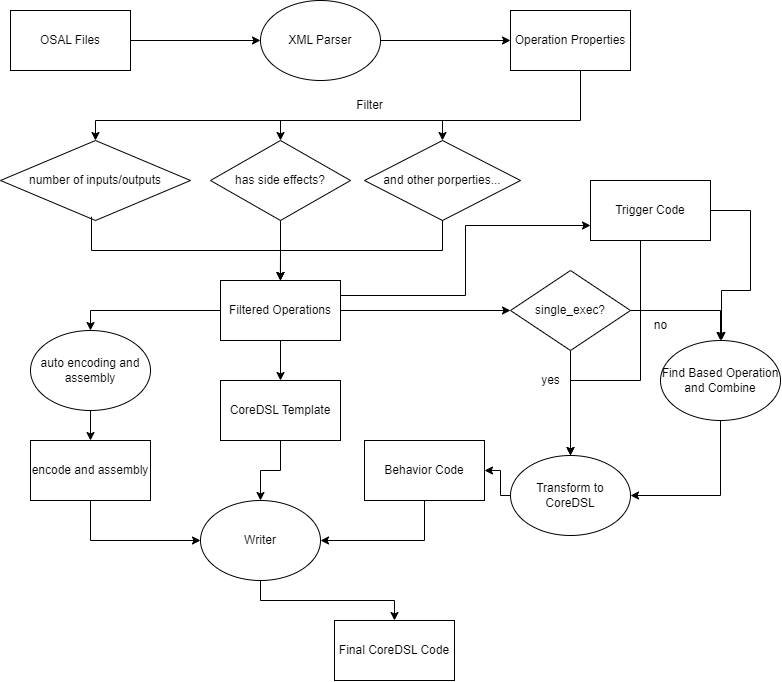
\includegraphics[width=\linewidth]{figures/flow.png}
  \caption{Implementation Flow}
\end{figure}

\section{XML Parser}

The process begins with the input OSAL (Operation Set Architecture Language) files, which contain the operation definitions. OpenASIP uses XML to define the properties and semantics of custom operations. To translate these operations into CoreDSL, we need to parse the XML representation and extract the necessary information. We developed an XML parser based on the \texttt{pandas} package in Python to read the XML files and extract the operation details.

The parser utilizes an object-oriented approach to ensure modularity and scalability. The extracted data is stored in the form of \texttt{pandas} DataFrames, which allows for efficient manipulation and filtering of the operations in the subsequent stages of processing. This structure provides flexibility for further operations, such as filtering based on input/output parameters or other properties, as required by the translation process.

\section{Operation Filtering}

The next stage involves filtering the operations based on predefined criteria. This step is crucial for identifying the operations that are suitable for further processing and transformation into CoreDSL code. The filtering process is designed to select operations that meet specific requirements, such as the number of inputs and outputs, the presence of side effects, or other characteristics that are relevant for the translation process.

\section{CoreDSL Template Generation}

The generation of the CoreDSL template involves several key steps. First, an empty CoreDSL template is created, which serves as the scaffold for defining the behavior of the custom operations. Then, the program iterates over the \textit{filtered operations} and fills in the necessary details into the template. The generation process leverages the parsed information from the XML files, including operation-specific attributes such as the number of input and output registers. The custom instructions are automatically encoded based on their properties, and the corresponding assembly code is generated.

\begin{lstlisting}[caption={CoreDSL Template},captionpos=b]
  InstructionSet OpenASIP_base extends RV32I {
    functions{
        // Inline functions for behavior
    }
    instructions {
        // Example for custom instruction
        OpenASIP_base_SHL1ADD {
            encoding: 7'b0000000 :: rs2[4:0] :: rs1[4:0] :: 3'b000 :: rd[4:0] :: 7'b0001011;
            assembly: "{name(rd)}, {name(rs1)}, {name(rs2)}";
            behavior: {
                // Behavior code will be generated here
            }
        }
        // Additional instructions will be iteratively generated
    }
  }
\end{lstlisting}

\subsection{Inline Function}

The inline functions required for custom operations are defined as part of the \textit{trigger codes} within the OpenASIP framework. Although OpenASIP provides the trigger code definition, it does not include the actual implementation of these inline functions. Fortunately, these functions are relatively simple to implement and are inserted at the beginning of the CoreDSL file. This ensures that all behavior code for custom instructions can utilize these functions during execution.

\subsection{Auto Encoding and Assembly}

The encoding process for custom instructions is handled automatically by the program. As the filtered operations are processed sequentially, each instruction is assigned an encoding that follows the RISC-V extension format. For example, instructions with two input registers (\texttt{rs1} and \texttt{rs2}) and one output register (\texttt{rd}) will be encoded in a standard 32-bit RISC-V format.

For assembly code generation, the program analyzes the XML-defined instruction attributes, such as the number of source and destination registers. Based on these attributes, it generates the corresponding assembly format string, ensuring that the generated assembly matches the intended behavior of each instruction. The following example shows how the registers are referenced in the assembly code:

\begin{lstlisting}
  assembly: "{name(rd)}, {name(rs1)}, {name(rs2)}";
\end{lstlisting}

This ensures that all operations are properly defined within the CoreDSL framework, both at the encoding level and in terms of their assembly representation.

\section{Behavior Code Generation}

The generation of behavior code for custom operations is a crucial step in translating operation semantics into executable instructions within the CoreDSL framework. This process primarily revolves around interpreting the trigger semantics provided for each operation and converting them into behavior code that can be executed by the target architecture.

\subsection{Handling \texttt{single\_execute} Operations}

Operations classified as \texttt{single\_execute} are those that involve zero or exactly one \texttt{EXEC\_OPERATION}. These operations are simpler to handle, as their semantics are either minimal or require only a single execution step. The process of generating behavior code for \texttt{single\_execute} operations is as follows:

\begin{enumerate}
    \item \textbf{Search for Trigger Code}: The program first attempts to locate the corresponding trigger code from the parsed operation semantics. This code typically contains the behavior definition for the operation.

    \item \textbf{Fallback for Missing Trigger Code}: If the trigger code is not found, the program uses a fallback approach. In this case, the tool looks for a base operation (i.e., a related or parent operation) that shares similar functionality. If a base operation is identified, its behavior code is transformed and reused. If no such base operation is available, a warning is issued, and the behavior code is generated as a placeholder or default behavior, depending on the requirements of the architecture.

    \item \textbf{Example}:
    \begin{lstlisting}
        // Example of a fallback behavior code for a missing trigger
        X[rd % RFS] = X[rs1 % RFS] + X[rs2 % RFS]; // Default operation: addition
    \end{lstlisting}
\end{enumerate}

This approach ensures that even when the exact semantics are not available, the system can still produce a working instruction that adheres to general operation principles.

\subsection{Handling Different Variable Names}

In some cases, variable names in the trigger code might differ from the expected format used in the CoreDSL framework. This is a common issue, especially when operations are defined in different contexts or environments. The tool handles this issue by:

\begin{enumerate}
    \item \textbf{Pattern Matching and Variable Mapping}: The tool applies pattern matching to identify variables in the trigger code (e.g., \texttt{rs1}, \texttt{rs2}, \texttt{rd}) and maps them to the expected format used in the target architecture. This ensures consistency in variable naming across all operations.

    \item \textbf{Renaming Strategy}: If the trigger code uses custom variable names (e.g., \texttt{temp\_reg} or \texttt{intermediate\_value}), the tool automatically replaces these with the standard naming convention used in CoreDSL (such as \texttt{X[rs1]}, \texttt{X[rs2]}, \texttt{X[rd]}). This is done using regular expressions to match and substitute variable names accordingly.

    \item \textbf{Example}:
    \begin{lstlisting}
        // Before transformation: uses custom variable names
        temp_reg = X[rs1] + X[rs2];
        intermediate_value = temp_reg * 2;

        // After transformation: standard variable names
        X[rd % RFS] = X[rs1 % RFS] + X[rs2 % RFS];
        X[rd % RFS] = X[rd % RFS] * 2;
    \end{lstlisting}
\end{enumerate}

This automatic renaming ensures that all behavior code conforms to the same format, regardless of the original trigger code's naming conventions.

\subsection{Handling Missing or Incomplete Trigger Code}

There are cases where the provided trigger code is incomplete or missing certain details, such as variable initialization or conditional checks. To handle these situations, the tool applies several strategies:

\begin{enumerate}
    \item \textbf{Default Values for Missing Variables}: If a required variable is missing or uninitialized in the trigger code, the tool inserts default values or initialization based on the context of the operation. For instance, if a result register (\texttt{rd}) is not initialized, it may be set to a default value like zero or an identity element (e.g., 1 for multiplication).

    \item \textbf{Handling Conditional Logic}: If the trigger code includes conditional statements (e.g., \texttt{if} conditions) without complete implementation, the tool generates the necessary control flow structures. For example, if a condition involves checking the value of a register, the tool ensures that the check is properly implemented and that the code handles both the true and false branches.

    \item \textbf{Example}:
    \begin{lstlisting}
        // Incomplete conditional logic
        if (X[rs2] == 0) {
            // Missing else branch
        }

        // Completed by the tool
        if (X[rs2 % RFS] == 0) {
            X[rd % RFS] = 0;  // Handle divide by zero
        } else {
            X[rd % RFS] = X[rs1 % RFS] / X[rs2 % RFS];  // Normal division
        }
    \end{lstlisting}
\end{enumerate}

By filling in missing parts of the code, the tool ensures that the behavior of the instruction remains consistent and functional.

\subsection{Handling Other Corner Cases}

In addition to the common cases mentioned above, the tool also addresses several corner cases that may arise during behavior code generation:

\begin{enumerate}
    \item \textbf{Multiple \texttt{EXEC\_OPERATION} Cases}: If an operation involves multiple \texttt{EXEC\_OPERATION} statements, the tool concatenates the behavior of these operations, ensuring that all steps are executed in the correct order. For example, if an operation involves both a shift and an addition, the tool ensures that both operations are included in the final behavior code.

    \item \textbf{Complex Trigger Semantics}: For operations with complex trigger semantics (e.g., involving multiple registers or advanced arithmetic operations), the tool decomposes the trigger code into manageable steps and generates the corresponding behavior code. This may involve splitting a single line of code into multiple steps to ensure clarity and correctness.

    \item \textbf{Error Handling}: In situations where runtime errors are defined (e.g., division by zero), the tool ensures that appropriate error handling mechanisms are inserted into the behavior code. This includes raising errors or returning safe default values when an error condition is detected.
\end{enumerate}

\subsection{Final Behavior Code Generation}

The final behavior code is generated by combining the transformed trigger code, any required fallback operations, and additional corner case handling. This ensures that each operation is fully defined within the CoreDSL framework and can be executed correctly on the target architecture. The behavior code is then inserted into the CoreDSL template, completing the generation process.

\begin{lstlisting}
// Example of final behavior code
if (X[rs2 % RFS] == 0) {
    X[rd % RFS] = 0;  // Handle divide by zero
} else {
    X[rd % RFS] = X[rs1 % RFS] / X[rs2 % RFS];
}
X[rd % RFS] = X[rd % RFS] + 1;  // Additional operation
\end{lstlisting}

This process ensures that all custom operations are correctly implemented and optimized for their respective architectures, regardless of the complexity of the trigger semantics or the specific requirements of the operation.


\chapter{Evaluation}
main results

\chapter{Conclusion}
\section{Conclusion}

In this work, we evaluated the integration and performance of custom instructions from the OpenASIP 2.0 Co-Design toolchain within the ETISS simulation framework. Using the CoreDSL ecosystem, we successfully translated custom OpenASIP operations into a format compatible with ETISS and tested these instructions using the MLonMCU benchmark suite.

The evaluation demonstrated that the custom instructions, while not dominating the overall execution, contributed specific enhancements in operations such as shifts and multiplications. Although the relative performance gains in terms of reduced instruction count and clock cycles were modest, this study highlights the potential for custom instructions to optimize embedded system performance, particularly in applications that can exploit specific custom operations.

Furthermore, the use of M2-ISA-R as a testing and debugging tool proved invaluable in identifying and correcting errors during the code generation process, allowing for an iterative development approach that ensured compatibility with the ETISS platform. The seamless integration of custom instructions and the observed performance metrics suggest that, with further refinement and targeting of specific workloads, significant optimizations can be achieved.

Future work will focus on extending the range of custom operations and evaluating their impact on more complex machine learning models and workloads. Additionally, more aggressive optimizations in both the instruction set and the ETISS simulation platform can be explored to maximize the performance benefits of custom instruction sets for embedded applications.

In summary, this study provides a foundational step toward enhancing embedded system performance through custom ISA extensions, and demonstrates the practicality of using tools like M2-ISA-R and ETISS to evaluate and benchmark these enhancements.

\backmatter
\bibliographystyle{plain}
\bibliography{chapters/references}

\end{document}
